\documentclass[sigplan,screen]{acmart}
\usepackage{graphicx}
\usepackage{fancybox}
\usepackage{listings}
\usepackage{xcolor}
\usepackage{subcaption}
\usepackage{setspace}
\usepackage{enumitem}

\newcommand{\nip}[1]{\vspace{1ex}\noindent\textbf{#1}}

\definecolor{ballblue}{rgb}{0.13, 0.67, 0.8}
\definecolor{bondiblue}{rgb}{0.0, 0.58, 0.71}
\definecolor{cobalt}{rgb}{0.0, 0.28, 0.67}
\definecolor{copper}{rgb}{0.72, 0.45, 0.2}
\definecolor{darkblue}{rgb}{0.0, 0.0, 0.55}
\definecolor{darkspringgreen}{rgb}{0.09, 0.45, 0.27}
\definecolor{gray}{gray}{0.5}
\definecolor{LightGray}{gray}{0.85}
\definecolor{VeryLightGray}{gray}{0.90}
\definecolor{ForestGreen}{rgb}{0.13, 0.55, 0.13}
\definecolor{Maroon}{rgb}{0.5, 0.0, 0.0}

\newcommand{\para}[1]{\smallskip\noindent {\bf #1} }
%\newcommand{\new}[1]{\textcolor{red}{#1}}
\newcommand{\comments}[1]{}

\iftrue   % toggle iftrue or iffalse
\newcommand{\tianyin}[1]{{{\color{red} [ty: #1]}}}
\newcommand{\jinghao}[1]{{\color{cyan} Jinghao: #1}}
\newcommand{\juowen}[1]{{\color{gray} Ruowen: #1}}
\newcommand{\djw}[1]{{\color{red}{\em (djw: #1)}}}
\newcommand{\raj}[1]{{\color{red}{\em (raj: #1)}}}
\newcommand{\mvle}[1]{{\color{darkblue}{\em (mvle: #1)}}}
\newcommand{\milo}[1]{{\color{orange}{\em (milo: #1)}}}
\newcommand{\hubertus}[1]{{\color{orange}{\em (frankeh: #1)}}}
\else
\newcommand{\tianyin}[1]{}
\newcommand{\jinghao}[1]{}
\newcommand{\juowen}[1]{}
\newcommand{\djw}[1]{}
\newcommand{\raj}[1]{}
\newcommand{\mvle}[1]{}
\newcommand{\milo}[1]{}
\newcommand{\hubertus}[1]{}
\fi

% \newcommand{\projname}{\textsf{R{\footnotesize E}X}}
\newcommand{\projname}{Rex}
\newcommand{\gap}{language-verifier gap}

%From https://github.com/denki/listings-rust/blob/master/listings-rust.sty
\lstdefinelanguage{Rust}{%
  sensitive%
, morecomment=[l]{//}%
, morecomment=[s]{/*}{*/}%
, moredelim=[s][{\itshape\color[rgb]{0,0,0.75}}]{\#[}{]}%
, morestring=[b]{"}%
, alsodigit={}%
, alsoother={}%
, alsoletter={!}%
%
%
% [1] reserve keywords
% [2] traits
% [3] primitive types
% [4] type and value constructors
% [5] identifier
%
, morekeywords={break, continue, else, for, if, in, loop, match, return, while}  % control flow keywords
, morekeywords={as, const, let, move, mut, ref, static}  % in the context of variables
, morekeywords={dyn, enum, fn, impl, Self, self, struct, trait, type, union, use, where}  % in the context of declarations
, morekeywords={crate, extern, mod, pub, super}  % in the context of modularisation
, morekeywords={unsafe}  % markers
, morekeywords={abstract, alignof, become, box, do, final, macro, offsetof, override, priv, proc, pure, sizeof, typeof, unsized, virtual, yield}  % reserved identifiers
%
% grep 'pub trait [A-Za-z][A-Za-z0-9]*' -r . | sed 's/^.*pub trait \([A-Za-z][A-Za-z0-9]*\).*/\1/g' | sort -u | tr '\n' ',' | sed 's/^\(.*\),$/{\1}\n/g' | sed 's/,/, /g'
, morekeywords=[2]{Add, AddAssign, Any, AsciiExt, AsInner, AsInnerMut, AsMut, AsRawFd, AsRawHandle, AsRawSocket, AsRef, Binary, BitAnd, BitAndAssign, Bitor, BitOr, BitOrAssign, BitXor, BitXorAssign, Borrow, BorrowMut, Boxed, BoxPlace, BufRead, BuildHasher, CastInto, CharExt, Clone, CoerceUnsized, CommandExt, Copy, Debug, DecodableFloat, Default, Deref, DerefMut, DirBuilderExt, DirEntryExt, Display, Div, DivAssign, DoubleEndedIterator, DoubleEndedSearcher, Drop, EnvKey, Eq, Error, ExactSizeIterator, ExitStatusExt, Extend, FileExt, FileTypeExt, Float, Fn, FnBox, FnMut, FnOnce, Freeze, From, FromInner, FromIterator, FromRawFd, FromRawHandle, FromRawSocket, FromStr, FullOps, FusedIterator, Generator, Hash, Hasher, Index, IndexMut, InPlace, Int, Into, IntoCow, IntoInner, IntoIterator, IntoRawFd, IntoRawHandle, IntoRawSocket, IsMinusOne, IsZero, Iterator, JoinHandleExt, LargeInt, LowerExp, LowerHex, MetadataExt, Mul, MulAssign, Neg, Not, Octal, OpenOptionsExt, Ord, OsStrExt, OsStringExt, Packet, PartialEq, PartialOrd, Pattern, PermissionsExt, Place, Placer, Pointer, Product, Put, RangeArgument, RawFloat, Read, Rem, RemAssign, Seek, Shl, ShlAssign, Shr, ShrAssign, Sized, SliceConcatExt, SliceExt, SliceIndex, Stats, Step, StrExt, Sub, SubAssign, Sum, Sync, TDynBenchFn, Terminal, Termination, ToOwned, ToSocketAddrs, ToString, Try, TryFrom, TryInto, UnicodeStr, Unsize, UpperExp, UpperHex, WideInt, Write}
, morekeywords=[2]{Send}  % additional traits
%
, morekeywords=[3]{bool, char, f32, f64, i8, i16, i32, i64, isize, str, u8, u16, u32, u64, unit, usize, i128, u128}  % primitive types
%
, morekeywords=[4]{Err, false, None, Ok, Some, true}  % prelude value constructors
% grep 'pub \(type\|struct\|enum\) [A-Za-z][A-Za-z0-9]*' -r . | sed 's/^.*pub \(type\|struct\|enum\) \([A-Za-z][A-Za-z0-9]*\).*/\2/g' | sort -u | tr '\n' ',' | sed 's/^\(.*\),$/{\1}\n/g' | sed 's/,/, /g'
, morekeywords=[3]{AccessError, Adddf3, AddI128, AddoI128, AddoU128, ADDRESS, ADDRESS64, addrinfo, ADDRINFOA, AddrParseError, Addsf3, AddU128, advice, aiocb, Alignment, AllocErr, AnonPipe, Answer, Arc, Args, ArgsInnerDebug, ArgsOs, Argument, Arguments, ArgumentV1, Ashldi3, Ashlti3, Ashrdi3, Ashrti3, AssertParamIsClone, AssertParamIsCopy, AssertParamIsEq, AssertUnwindSafe, AtomicBool, AtomicPtr, Attr, auxtype, auxv, BackPlace, BacktraceContext, Barrier, BarrierWaitResult, Bencher, BenchMode, BenchSamples, BinaryHeap, BinaryHeapPlace, blkcnt, blkcnt64, blksize, BOOL, boolean, BOOLEAN, BoolTrie, BorrowError, BorrowMutError, Bound, Box, bpf, BTreeMap, BTreeSet, Bucket, BucketState, Buf, BufReader, BufWriter, Builder, BuildHasherDefault, BY, BYTE, Bytes, CannotReallocInPlace, cc, Cell, Chain, CHAR, CharIndices, CharPredicateSearcher, Chars, CharSearcher, CharsError, CharSliceSearcher, CharTryFromError, Child, ChildPipes, ChildStderr, ChildStdin, ChildStdio, ChildStdout, Chunks, ChunksMut, ciovec, clock, clockid, Cloned, cmsgcred, cmsghdr, CodePoint, Color, ColorConfig, Command, CommandEnv, Component, Components, CONDITION, condvar, Condvar, CONSOLE, CONTEXT, Count, Cow, cpu, CRITICAL, CStr, CString, CStringArray, Cursor, Cycle, CycleIter, daddr, DebugList, DebugMap, DebugSet, DebugStruct, DebugTuple, Decimal, Decoded, DecodeUtf16, DecodeUtf16Error, DecodeUtf8, DefaultEnvKey, DefaultHasher, dev, device, Difference, Digit32, DIR, DirBuilder, dircookie, dirent, dirent64, DirEntry, Discriminant, DISPATCHER, Display, Divdf3, Divdi3, Divmoddi4, Divmodsi4, Divsf3, Divsi3, Divti3, dl, Dl, Dlmalloc, Dns, DnsAnswer, DnsQuery, dqblk, Drain, DrainFilter, Dtor, Duration, DwarfReader, DWORD, DWORDLONG, DynamicLibrary, Edge, EHAction, EHContext, Elf32, Elf64, Empty, EmptyBucket, EncodeUtf16, EncodeWide, Entry, EntryPlace, Enumerate, Env, epoll, errno, Error, ErrorKind, EscapeDebug, EscapeDefault, EscapeUnicode, event, Event, eventrwflags, eventtype, ExactChunks, ExactChunksMut, EXCEPTION, Excess, ExchangeHeapSingleton, exit, exitcode, ExitStatus, Failure, fd, fdflags, fdsflags, fdstat, ff, fflags, File, FILE, FileAttr, filedelta, FileDesc, FilePermissions, filesize, filestat, FILETIME, filetype, FileType, Filter, FilterMap, Fixdfdi, Fixdfsi, Fixdfti, Fixsfdi, Fixsfsi, Fixsfti, Fixunsdfdi, Fixunsdfsi, Fixunsdfti, Fixunssfdi, Fixunssfsi, Fixunssfti, Flag, FlatMap, Floatdidf, FLOATING, Floatsidf, Floatsisf, Floattidf, Floattisf, Floatundidf, Floatunsidf, Floatunsisf, Floatuntidf, Floatuntisf, flock, ForceResult, FormatSpec, Formatted, Formatter, Fp, FpCategory, fpos, fpos64, fpreg, fpregset, FPUControlWord, Frame, FromBytesWithNulError, FromUtf16Error, FromUtf8Error, FrontPlace, fsblkcnt, fsfilcnt, fsflags, fsid, fstore, fsword, FullBucket, FullBucketMut, FullDecoded, Fuse, GapThenFull, GeneratorState, gid, glob, glob64, GlobalDlmalloc, greg, group, GROUP, Guard, GUID, Handle, HANDLE, Handler, HashMap, HashSet, Heap, HINSTANCE, HMODULE, hostent, HRESULT, id, idtype, if, ifaddrs, IMAGEHLP, Immut, in, in6, Incoming, Infallible, Initializer, ino, ino64, inode, input, InsertResult, Inspect, Instant, int16, int32, int64, int8, integer, IntermediateBox, Internal, Intersection, intmax, IntoInnerError, IntoIter, IntoStringError, intptr, InvalidSequence, iovec, ip, IpAddr, ipc, Ipv4Addr, ipv6, Ipv6Addr, Ipv6MulticastScope, Iter, IterMut, itimerspec, itimerval, jail, JoinHandle, JoinPathsError, KDHELP64, kevent, kevent64, KV, l4, LARGE, lastlog, launchpad, Layout, Lazy, lconv, Leaf, LeafOrInternal, Lines, LinesAny, LineWriter, linger, linkcount, LinkedList, load, locale, LocalKey, LocalKeyState, Location, lock, LockResult, loff, LONG, lookup, lookupflags, LookupHost, LPBOOL, LPBY, LPBYTE, LPCSTR, LPCVOID, LPCWSTR, LPDWORD, LPFILETIME, LPHANDLE, LPOVERLAPPED, LPPROCESS, LPPROGRESS, LPSECURITY, LPSTARTUPINFO, LPSTR, LPVOID, LPWCH, LPWIN32, LPWSADATA, LPWSAPROTOCOL, LPWSTR, Lshrdi3, Lshrti3, lwpid, M128A, mach, major, Map, mcontext, Metadata, Metric, MetricMap, mflags, minor, mmsghdr, Moddi3, mode, Modsi3, Modti3, MonitorMsg, MOUNT, mprot, mq, mqd, msflags, msghdr, msginfo, msglen, msgqnum, msqid, Muldf3, Mulodi4, Mulosi4, Muloti4, Mulsf3, Multi3, Mut, Mutex, MutexGuard, MyCollection, n16, NamePadding, NativeLibBoilerplate, nfds, nl, nlink, NodeRef, NoneError, NonNull, NonZero, nthreads, NulError, OccupiedEntry, off, off64, oflags, Once, OnceState, OpenOptions, Option, Options, OptRes, Ordering, OsStr, OsString, Output, OVERLAPPED, Owned, Packet, PanicInfo, Param, ParseBoolError, ParseCharError, ParseError, ParseFloatError, ParseIntError, ParseResult, Part, passwd, Path, PathBuf, PCONDITION, PCONSOLE, Peekable, PeekMut, Permissions, PhantomData, pid, Pipes, PlaceBack, PlaceFront, PLARGE, PoisonError, pollfd, PopResult, port, Position, Powidf2, Powisf2, Prefix, PrefixComponent, PrintFormat, proc, Process, PROCESS, processentry, protoent, PSRWLOCK, pthread, ptr, ptrdiff, PVECTORED, Queue, radvisory, RandomState, Range, RangeFrom, RangeFull, RangeInclusive, RangeMut, RangeTo, RangeToInclusive, RawBucket, RawFd, RawHandle, RawPthread, RawSocket, RawTable, RawVec, Rc, ReadDir, Receiver, recv, RecvError, RecvTimeoutError, ReentrantMutex, ReentrantMutexGuard, Ref, RefCell, RefMut, REPARSE, Repeat, Result, Rev, Reverse, riflags, rights, rlim, rlim64, rlimit, rlimit64, roflags, Root, RSplit, RSplitMut, RSplitN, RSplitNMut, RUNTIME, rusage, RwLock, RWLock, RwLockReadGuard, RwLockWriteGuard, sa, SafeHash, Scan, sched, scope, sdflags, SearchResult, SearchStep, SECURITY, SeekFrom, segment, Select, SelectionResult, sem, sembuf, send, Sender, SendError, servent, sf, Shared, shmatt, shmid, ShortReader, ShouldPanic, Shutdown, siflags, sigaction, SigAction, sigevent, sighandler, siginfo, Sign, signal, signalfd, SignalToken, sigset, sigval, Sink, SipHasher, SipHasher13, SipHasher24, Skip, SkipWhile, Slice, SmallBoolTrie, sockaddr, SOCKADDR, sockcred, Socket, SOCKET, SocketAddr, SocketAddrV4, SocketAddrV6, socklen, speed, Splice, Split, SplitMut, SplitN, SplitNMut, SplitPaths, SplitWhitespace, spwd, SRWLOCK, ssize, stack, STACKFRAME64, StartResult, STARTUPINFO, stat, Stat, stat64, statfs, statfs64, StaticKey, statvfs, StatVfs, statvfs64, Stderr, StderrLock, StderrTerminal, Stdin, StdinLock, Stdio, StdioPipes, Stdout, StdoutLock, StdoutTerminal, StepBy, String, StripPrefixError, StrSearcher, subclockflags, Subdf3, SubI128, SuboI128, SuboU128, subrwflags, subscription, Subsf3, SubU128, Summary, suseconds, SYMBOL, SYMBOLIC, SymmetricDifference, SyncSender, sysinfo, System, SystemTime, SystemTimeError, Take, TakeWhile, tcb, tcflag, TcpListener, TcpStream, TempDir, TermInfo, TerminfoTerminal, termios, termios2, TestDesc, TestDescAndFn, TestEvent, TestFn, TestName, TestOpts, TestResult, Thread, threadattr, threadentry, ThreadId, tid, time, time64, timespec, TimeSpec, timestamp, timeval, timeval32, timezone, tm, tms, ToLowercase, ToUppercase, TraitObject, TryFromIntError, TryFromSliceError, TryIter, TryLockError, TryLockResult, TryRecvError, TrySendError, TypeId, U64x2, ucontext, ucred, Udivdi3, Udivmoddi4, Udivmodsi4, Udivmodti4, Udivsi3, Udivti3, UdpSocket, uid, UINT, uint16, uint32, uint64, uint8, uintmax, uintptr, ulflags, ULONG, ULONGLONG, Umoddi3, Umodsi3, Umodti3, UnicodeVersion, Union, Unique, UnixDatagram, UnixListener, UnixStream, Unpacked, UnsafeCell, UNWIND, UpgradeResult, useconds, user, userdata, USHORT, Utf16Encoder, Utf8Error, Utf8Lossy, Utf8LossyChunk, Utf8LossyChunksIter, utimbuf, utmp, utmpx, utsname, uuid, VacantEntry, Values, ValuesMut, VarError, Variables, Vars, VarsOs, Vec, VecDeque, vm, Void, WaitTimeoutResult, WaitToken, wchar, WCHAR, Weak, whence, WIN32, WinConsole, Windows, WindowsEnvKey, winsize, WORD, Wrapping, wrlen, WSADATA, WSAPROTOCOL, WSAPROTOCOLCHAIN, Wtf8, Wtf8Buf, Wtf8CodePoints, xsw, xucred, Zip, zx}
%
, morekeywords=[5]{assert!, assert_eq!, assert_ne!, cfg!, column!, compile_error!, concat!, concat_idents!, debug_assert!, debug_assert_eq!, debug_assert_ne!, env!, eprint!, eprintln!, file!, format!, format_args!, include!, include_bytes!, include_str!, line!, module_path!, option_env!, panic!, print!, println!, select!, stringify!, thread_local!, try!, unimplemented!, unreachable!, vec!, write!, writeln!}  % prelude macros
, morekeywords=[6]{windows, enumerate, filter_map, iter, take_while, for_each}% Specific functions we used
, keywordstyle=\color{cobalt}% reserved keywords
, keywordstyle=[2]\color[rgb]{0.75, 0, 0}% traits
, keywordstyle=[3]\color[rgb]{0, 0.5, 0}% primitive types
, keywordstyle=[4]\color[rgb]{0, 0.5, 0}% type and value constructors
, keywordstyle=[5]\color[rgb]{0, 0, 0.75}% macros
, keywordstyle=[6]\color{blue}% Specific functions we used
, stringstyle=\color{copper}%
, basicstyle=\tiny\ttfamily%
, numbers=left%
, numbersep=6pt%
, numberstyle=\tiny\ttfamily\color{gray}%
, breaklines=true%
, escapeinside={(*@}{@*)}%
, showstringspaces=false%
, xleftmargin=8pt%
}%

\lstdefinelanguage{myC}[]{C}{
  morekeywords={assert},
  morecomment=[f][\color{blue}]{@@},     % group identifier
  morecomment=[f][\color{red}]-,         % deleted lines
  morecomment=[f][\color{ForestGreen}]+, % added lines
  morecomment=[f][\color{magenta}]{---}, % Diff header lines (must appear after +,-)
  morecomment=[f][\color{magenta}]{+++},
  morecomment=[f][\color{magenta}]{//},
  morecomment=[f][\color{magenta}]{/*},
  morecomment=[f][\color{magenta}]{\ \ \ \ //},
  morecomment=[f][\color{magenta}]{//},
  keywords = {DROP_POLICY_DENY, DROP_POLICY_AUTH_REQUIRED, CTX_ACT_OK,
    DROP_INVALID, BMC_MAX_PACKET_LENGTH, ENABLE_IPV4_FRAGMENTS,
    DROP_CT_INVALID_HDR, ENABLE_SRV6_SRH_ENCAP, IPPROTO_IPIP, IPPROTO_IPV6,
    ETH_HLEN, POLICY_MATCH_L4_ONLY, POLICY_MATCH_L3_PROTO, IS_ERR, likely,
    __always_inline, offsetof},
  keywords = [2]{long, int, u32, const, void, if, return, switch, return, case,
    break, u64, u8, unsigned, struct, sizeof, __u8, __s8, default, else, for,
    static, asm, volatile},
  keywordstyle=\color{purple},
  keywordstyle=[2]\color{blue},
  commentstyle=\color{darkspringgreen},
  stringstyle=\color{blue},
  numbers=left,
  basicstyle=\tiny\ttfamily,
  numbersep=6pt,
  numberstyle=\tiny\ttfamily\color{gray},
  breaklines=true,
  escapeinside={(*@}{@*)},
  showstringspaces=false,
  xleftmargin=8pt,
  %% postbreak=\mbox{\textcolor{red}{$\hookrightarrow$}\space},
}

\lstdefinelanguage{myBPF}[]{C}{
  morecomment=[f][\color{magenta}];,
  keywords = {r1, r2, r3, r4, r5, r6, r7, r8, r9, ctx, pkt,
    w1, w2, w3, w4, w5, w6, w7, w8, w9},
  keywords = [2]{u8, u16, u32, u64},
  keywordstyle=\color{purple},
  keywordstyle=[2]\color{blue},
  commentstyle=\color{darkspringgreen},
  stringstyle=\color{blue},
  numbers=left,
  basicstyle=\tiny\ttfamily,
  numbersep=6pt,
  numberstyle=\tiny\ttfamily\color{gray},
  breaklines=true,
  escapeinside={(*@}{@*)},
  showstringspaces=false,
  xleftmargin=8pt,
  %% postbreak=\mbox{\textcolor{red}{$\hookrightarrow$}\space},
}


%%
%% \BibTeX command to typeset BibTeX logo in the docs
\AtBeginDocument{%
  \providecommand\BibTeX{{%
    Bib\TeX}}}


%%
%% end of the preamble, start of the body of the document source.
\begin{document}

%%
%% The "title" command has an optional parameter,
%% allowing the author to define a "short title" to be used in page headers.
\title{Inner-unikernels}

%%
%% The "author" command and its associated commands are used to define
%% the authors and their affiliations.
%% Of note is the shared affiliation of the first two authors, and the
%% "authornote" and "authornotemark" commands
%% used to denote shared contribution to the research.

%%
%% By default, the full list of authors will be used in the page
%% headers. Often, this list is too long, and will overlap
%% other information printed in the page headers. This command allows
%% the author to define a more concise list
%% of authors' names for this purpose.

%%
%% The abstract is a short summary of the work to be presented in the
%% article.
\begin{abstract}
    TODO
\end{abstract}


%%
%% The code below is generated by the tool at http://dl.acm.org/ccs.cfm.
%% Please copy and paste the code instead of the example below.
%%

%%
%% Keywords. The author(s) should pick words that accurately describe
%% the work being presented. Separate the keywords with commas.

%%
%% This command processes the author and affiliation and title
%% information and builds the first part of the formatted document.
\maketitle

\section{Introduction}

\begin{itemize}
    \item eBPF is the de-facto way of doing kernel extension in Linux
    \item Used in different domains
    \item
        \begin{itemize}
            \item networking, tracing, security
            \item also embraced by research community (BMC, XRP, Electrode)
        \end{itemize}
    \item Core value argument: verification for safety
    \item Problem: current static verification scheme (i.e. the verifier)
        places unnecessary constraints on expressiveness on extension programs
        \begin{itemize}
            \item BMC has a subsection discussing verification workarounds
            \item We had an unpleasant experience in porting BMC (though this
                is more like the new compiler does not play well with the
                verifier for some old code)
            \item Overhead argument in BMC (sending data through map vs
                function arguments)
            \item Certain program constructs are not possible
            \item Some more evidence/example needed
        \end{itemize}
    \item Another point to include: for certain safety properties static
        verification is fundamentally limited even in current eBPF
        \begin{itemize}
            \item From Roop's experiment: there is not a way for verifier to
                figure out statically how much stack will be used when bpf2bpf
                calls and tail calls are mixed due to the indirect nature of
                tail calls. If the stack is 8k (e.g. on 32-bit platforms) the
                verifier cannot protect the stack.
            \item Related to our argument on runtime mechanism
        \end{itemize}
    \item Our solution: we should use a more expressive language for kernel
        extensions and move away from the verifier. The language should:
        \begin{itemize}
            \item be more expressive (e.g. Turing complete)
            \item support equivalent safety properties as the verifier (the
                hotos table)
                \begin{itemize}
                    \item memory safety
                    \item control-flow safety
                    \item type safety
                    \item safe resource management
                    \item program termination
                    \item kernel stack overflow protection
                \end{itemize}
            \item Rust
                \begin{itemize}
                    \item a widely used high-level programming language, also
                        embraced by Linux (Rust for Linux)
                    \item happens to have most of these properties out-of-box,
                        therefore we choose to build upon Rust
                \end{itemize}
        \end{itemize}
\end{itemize}
\section{Background: Safe Kernel Extensions}
\label{sec:background}
\djw{thinking about this being ``background and motivation'' with this being the first half and 3 being the section half}

%% \subsection{eBPF}
%% eBPF is a Linux kernel subsystem that allows for safe and dynamic kernel extension.
%% Developers write programs that get compiled to eBPF bytecode before being verified by an in-kernel verifier.
%% The verifier ensures certain safety properties about the programs such as termination and memory safety.
%% The execution of eBPF programs follows an event based mechanism, where control flow will transfer to the extension when certain events happen in the system.
%% eBPF programs also have access to a set of helper functions inside the kernel, which allow them to interact with kernel state.
%% Recent work has argued that the safety guarantees of the eBPF verifier are not as strong as claimed, especially in respect to the helper function interface \cite{untenableVerification}.

%% %\begin{itemize}
%% %    \item extension program model
%% %    \item verification
%% %    \item helpers
%% %    \item eBPF problems, echo the HotOS paper
%% %\end{itemize}

%% \subsection{Rust}

%% \juowen{TODO: maybe add some content related to Rust's syntactic sugar}
%% \begin{itemize}
%%     \item language-based safety
%%     \item expressiveness
%% \end{itemize}
%% \hubertus{you have to describe what "safe Rust" vs. "regular Rust" is, you should also highlight the popularity of Rust "https://medium.com/@codilime/the-future-of-rust-characteristics-popularity-and-challenges-7de4db5ebd67"}
%% % \subsection{Rust v.s. eBPF}
%% %
%% % \begin{itemize}
%% %     \item Probably has a better place
%% %     \item Sets and examples we discussed
%% %         \begin{itemize}
%% %             \item Rust and eBPF: Small, simple programs
%% %             \item eBPF but not Rust: certain code is unsafe in Rust but safe in
%% %                 eBPF, e.g. reinterpreting bytes in a packet into another struct
%% %             \item Rust but not eBPF: Expressiveness argument
%% %         \end{itemize}
%% % \end{itemize}


%% \subsection{Threat Model for Safe Kernel Extensions}
%% Part of the success of eBPF in the industry stems from its claim of
%% safety, achieved by the in-kernel verifier.  For example, as opposed
%% to Linux kernel modules (written in C), safety in eBPF lowers the
%% barrier to entry and trust required for system administrators to
%% install an extension into a production system.  However, there are
%% ongoing debates in industry~\cite{unprivileged-ebpf} and
%% academia~\cite{untenableVerification} about the quality of eBPF's safety
%% guarantees and in what circumstances they can be relied on.  Here we
%% specify the threat model and expectations for safety of kernel
%% extensions for the scope of this paper.

%% We assume that extensions are installed by a system administrator with
%% root privileges on the system.  Extensions are written by well-meaning
%% but imperfect developers and thus may contain programming mistakes.
%% We assume that the extension is not actively malicious.  So called
%% ``guarantees'' of safety therefore consist of the best-effort catching
%% of common mistakes.  While some in the community may be interested in
%% exploring stronger notions of
%% safety~\cite{unprivileged-ebpf,jia2023}, we note that this
%% definition of safety is consistent with the current eBPF ecosystem,
%% where actively malicious extension writers can crash or hang the
%% system~\cite{untenableVerification,ebpf-stackoverflow,ebpf-termination} (e.g.,
%% via helper functions), but the verifier prevents obvious mistakes (e.g.,
%% dereferencing a NULL pointer).




Kernel extensions allow code to be added to the kernel dynamically at
runtime for use cases ranging from observability and monitoring to
customization and acceleration.  Whereas safety of extensions was once
only a concern of the research community (e.g., SPIN~\cite{spin},
VINO~\cite{vino}, etc.), the shortening space between development,
debugging and deployment in today's industry landscape has created a
need for extending systems in production, where any system instability
caused by extensions is difficult to tolerate.

As a result, the past decade has seen the re-emergence of safety
concerns for kernel extensions, embodied in Linux by the eBPF
ecosystem.  Unlike the Linux kernel module framework, where modules
are written in C and programmer errors (e.g., errant pointer
dereferences, integer overflows) will crash the kernel, the eBPF
framework attempts to limit the damage from extension programmer error
by compiling extensions written in a high-level language like C or
Rust to a bytecode representation that is checked at extension load
time by an in-kernel verifier.  This workflow is shown in
Figure~\ref{fig:gap}.

%% \begin{figure}
%%     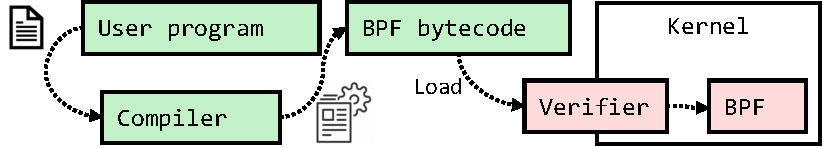
\includegraphics[width=1.0\linewidth]{figs/bpf_intro.pdf}
%%     \centering
%%     \vspace{-10pt}
%%     \caption{Overview of eBPF}
%%     \label{fig:ebpf}
%%     \vspace{-10pt}
%% \end{figure}

The safety properties checked by the eBPF verifier are generally
related to avoiding kernel crashes or hangs.  In eBPF, the verifier
uses a form of symbolic execution on the bytecode to examine all
possible executions to ensure safety.  It also performs limited
checks on the extension's
interactions with the kernel through {\em
  helper functions}.
We characterize these verifier
checks as ensuring the following conceptual properties of the
extension:
\begin{itemize}
\item {\bf Memory Safety:} Extensions can only access memory that is
  provided to them through explicit context arguments or kernel
  interfaces, (e.g., helper functions).  This prevents kernel crashes
  through NULL pointer dereference or corruption of kernel data
  structures.
\item {\bf Type Safety:} When accessing data in memory, the extension must use
  the correct type of the data. This helps avoid misinterpretation of the data
  or memory corruptions.
% When invoking kernel interfaces, the
%   extension must supply arguments of the appropriate type.  This helps
%   avoid kernel crashes in helper functions.
\item {\bf Resource Safety:} When gaining access to kernel objects
  (e.g., lock, allocated memory, etc.) through helper function,
  extensions must subsequently invoke the appropriate release
  interface on the object before completion.  This prevents memory
  leaks or deadlocks that can hang or crash the kernel.
\item {\bf Runtime Safety:} Extensions must terminate. This prevents
  infinite loops that hang the kernel indefinitely.
\item {\bf Undefined Behavior Elimination:} Extensions must never
  exhibit undefined behavior, including integer errors (e.g.,
  overflow, divide by zero, etc.). This prevents runtime kernel
  crashes.
\item {\bf Stack safety:} A unique safety requirement for kernel exntensions.
  Extension must not overflow the limited kernel stack.
  Failing to do so risks kernel crashes or kernel memory corruption.
\end{itemize}

This notion of safety in eBPF lowers the barrier to entry and trust
required for system administrators to install an extension into a
production system.  However, there are ongoing debates in
industry~\cite{reconsider-unpriv-ebpf-lwn,seccomp-ebpf-lwn,ebpf-sec-lwn} and
academia~\cite{untenableVerification} about the quality of eBPF's
safety guarantees and in what circumstances they can be relied on.
Here we specify the safety model and expectations for safety of kernel
extensions for the scope of this paper.

\paragraph{Safety model:} We assume that extensions are installed by a system administrator with
root privileges on the system.  Extensions are written by well-meaning
but imperfect developers and thus may contain programming mistakes.
We assume that the extension is not actively malicious.  So called
``guarantees'' of safety therefore consist of the best-effort catching
of common mistakes.  While some in the community may be interested in
exploring stronger notions of safety~\cite{reconsider-unpriv-ebpf-lwn,seccomp-ebpf-lwn,ebpf-sec-lwn,jia2023},
we note that this definition of safety is consistent with the current
eBPF ecosystem, where actively malicious extension writers can crash
or hang the
system~\cite{untenableVerification,ebpf-stackoverflow,ebpf-termination}
(e.g., via helper functions), but the verifier prevents obvious
mistakes (e.g., dereferencing a NULL pointer).

\section{Design}

\section{Design and Implementation}

\subsection{Design goal}

%\begin{itemize}
%     \item Safety
%         \begin{itemize}
%             \item Same level of safety as eBPF
%             \item Memory safety
%             \item Control-flow soundness
%             \item Resource management
%             \item Program termination
%         \end{itemize}
%     \item Expressiveness
%         \begin{itemize}
%             \item Support more complicated/advanced programs
%             \item Longer programs
%             \item Unbounded loops
%         \end{itemize}
%     \item An important note: we want expressiveness w/o impairing safety (e.g.
%         allow unbounded loop while ensuring termination)
% \end{itemize}

\subsection{Overview}
\begin{itemize}
    \item Brings out the Rust based approach (use Jiyuan's property-oriented
        argument: We want these properties, and Rust happens to provide these)
    \item Infrastructure (Need a figure similar to Fig. 5 from HotOS paper)
\end{itemize}

\subsection{Program load and attachment}
\begin{itemize}
    \item kernel loading code and attachment
    \item relocation fixups for maps and kernel symbols
    \item libiu
\end{itemize}

\subsection{Runtime crate as the programming interface}
\begin{itemize}
    \item overall structure: program type, kernel binding generation, wrapper
        interface around binding.
    \item kernel helper and symbol bindings (dynamic linking scheme)
    \item kconfig-based conditional compilation
\end{itemize}

\para{Kernel symbol resolution}
The \projname{} kernel crate serves as an interface for the extension programs
    to interact with the kernel.
To accomplish this, the crate will need to access kernel symbols.
For example, invoking kernel helper functions requires knowing the kernel
    address of the target helper function symbol.
These kernel symbols includes not only BPF helper functions, but also other
    global and per-CPU variables.

Because \projname{} programs are compiled in userspace, the compiler does not
    have knowledge on any of the required kernel symbols.
One simple solution is to directly passing kernel symbols and their
    corresponding addresses to userspace (e.g. through \texttt{/proc/kallsyms})
However, this is in general considered a dangerous practice as it leaks kernel
    addresses to userspace.
At the same time, this solution is not robust against kernel layout changes
    (e.g. due to kernel rebuild) -- changes of a kernel symbol address requires
    a recompilation of the \projname{} program that uses it.

Our implementation defers the kernel symbol resolution to program load time,
    i.e. when the compiled \projname{} program is sent to the kernel.
At this point, the booted kernel always knows where the symbols are located,
    even after layout changes.
At the same time, the sensitive kernel addresses do not need to be leaked to
    userspace.
\projname{} implements this kernel symbol resolution scheme the same way
    dynamic linking works in userspace.
The compilation process treats all kernel symbols as external and generate
    relocation entries for these undefined symbols.
At load time, the loader library parses the executable, compiles a list of
    kernel sybmols that require resolution with their corresponding entries in
    the global offset table (GOT), and sends the information to the kernel.
The kernel then resolves the address for each symbol via the kallsyms subsystem
    and patches the GOT entries with the resolved addresses and allows programs
    to correctly referencing these kernel symbols.

\para{Kconfig-aware conditional compilation}
% kernel uses config-based conditional compilation
% certain functionalities may not be compiled in
% we also use conditional compilation in kernel crate
% read config from build script and pass to the compilation process
The fact that the Linux kernel employs conditional compilation extensively
    based on kernel configuration values implies that certain functionalities
    used by \projname{} programs may not be compiled in.
An example of this is the ability to override the return value of a function in
    Kprobe programs.
This is only available if the \texttt{CONFIG\_BPF\_KPROBE\_OVERRIDE} is
    enabled.
The \projname{} kernel crate utilizes the conditional compilation counterpart
    in Rust.
The build script of the crate parses the configuration of the kernel for which
    the program is built and send configuration values of interest to the
    compiler.
If a functionality does not have its associated configuration set, its support
    in the kernel crate will not be present, either.

\subsection{Entry code generation}
\begin{itemize}
    \item LLVM pass
\end{itemize}

\subsection{Handle exceptional control flow}
\begin{itemize}
    \item kernel trampoline
\end{itemize}

\subsection{Stack overflow protection}
\begin{itemize}
    \item kernel vmapped, dedicated stack
    \item LLVM instrumentation
\end{itemize}

\subsection{program termination}
\begin{itemize}
    \item Need work
\end{itemize}

\section{Evaluation}

% \begin{itemize}
%     \item Macro-benchmark
%         \begin{itemize}
%             \item BMC
%                 \begin{itemize}
%                     \item Expressiveness: how to evaluate?
%                         \begin{itemize}
%                             \item LOC: we have 33\% reduction
%                             \item 1 rust program vs 7 eBPF programs
%                             \item based on experience?
%                             \item Rust is a safer language
%                         \end{itemize}
%                     \item Performance evaluation
%                         \begin{itemize}
%                             \item Check their paper to see if we can perform
%                                 the same experiment
%                             \item We want a figure similar to Figure 6 in BMC
%                                 (except we don't need to evaluate on different
%                                 CPU configs)
%                             \item x: Vanilla memcached, BMC, Rust
%                             \item y: normalized throughput
%
%                         \end{itemize}
%                 \end{itemize}
%             \item Electrode
%                 \begin{itemize}
%                     \item LOC reduction
%                     \item Performance using their benchmark (similar to figure
%                         5 and 7 in Electrode)
%                     \item Dynamic allocation (ask the authors)
%                 \end{itemize}
%             \item LSM implementation (if we have time / requires handle
%                 nesting)
%             \item XRP
%             \item FUSE in eBPF (from Hubertus)
%         \end{itemize}
%     \item Micro-benchmark
%         \begin{itemize}
%             \item Memory footprint (BPF vs Rust) given we have a larger binary
%                 \begin{itemize}
%                     \item Number of prog in the same translation unit vs memory
%                         usage for program allocation
%                     \item This is because we are always statically linked to
%                         the runtime crate on the translation unit basis
%                     \item E.g. a bpf kern.c with 4 programs vs a rust main.rs
%                         with 4 programs
%                 \end{itemize}
%             \item Small expressiveness examples
%                 \begin{itemize}
%                     \item Loop: strcmp
%                     \item need more
%                 \end{itemize}
%             \item Stack-check overhead
%                 \begin{itemize}
%                     \item Use BMC?
%                     \item Or create some other workload that are function call
%                         intensive (since our instrumentation happens before
%                         each function call)
%                 \end{itemize}
%             \item Cleanup overhead on normal execution path (recording
%                 allocated kernel objects)
%                 \begin{itemize}
%                     \item Similar to Stack-check
%                 \end{itemize}
%             \item Startup overhead due to stack switching
%                 \begin{itemize}
%                     \item A minimal program () to show the upper bound?
%                     \item Plus a real world application (again BMC)?
%                 \end{itemize}
%         \end{itemize}
% \end{itemize}

\subsection{Micro-benchmarks}
\subsubsection{Memory footprint (BPF vs Rust)}
% definition of memory footprint
% eBPF only have JIT code
% Rust have code sections and other sections, e.g. data and GOT sections
We evaluate on how large the in-kernel memory footprint of \projname{} programs
    is comparing to that of eBPF programs.
We define the memory footprint as the number of static memory pages required
    for program execution.
For eBPF, this only includes the JIT-ed native code, since eBPF program does
    not support static data sections.
For \projname{} this includes all load segments from the compiled ELF
    executable, which consists not only the text sections, but also the data
    sections for static variables (e.g., program objects and maps objects) as
    well as the sections that implement support for position-independent code
    (e.g., GOT sections).

In this experiment, we compare the number of memeory pages required for both
    \projname{} programs and their equivalent eBPF programs.
We select 3 simple eBPF programs from the sample eBPF programs shipped with the
    kernel -- the trace point program \texttt{syscall\_tp}, the kprobe program
    \texttt{tracex5} and the perf event program \texttt{trace\_event}.
We also include the BMC program (\S~\ref{eval:macro}) in the experiment because
    it represents an example of a complicated eBPF program.
For all the programs, we implement a \projname{} version with the same
    overall logic.

\begin{itemize}
    \item need a figure: bar graph showing the memory footprint of bpf and
        \projname{} programs on our sample programs
    \item sample programs: \texttt{syscall\_tp}, \texttt{tracex5},
        \texttt{trace\_event}, and BMC.
    \item y: total number of pages allocated for the loaded object (JIT-ed code
        for BPF, loaded and mapped pages for Rust)
\end{itemize}

\jinghao{Discussion on the result really needs the result, I am not sure which
one will have a smaller memory footprint.}

\subsubsection{Startup overhead due to stack switching}
\begin{table}[t]
    \small
    \centering
    \begin{tabular}{cc}%{|p{6cm}|p{1cm}|}
        \toprule
        \textbf{Extension} & \textbf{Runtime of empty program (ns)} \\
        \midrule
        eBPF & 43.5 $\pm$ 4.79 \\
        \projname{} & 44.1 $\pm$ 4.93 \\
        \bottomrule
    \end{tabular}
    \caption{Runtime of an empty program for eBPF and \projname{}}
    \vspace{-10pt}
    \label{tab:startup-overhead}
\end{table}

\projname{}'s usage of a dedicated stack for execution and the implementation
    of exception handling support may incur additional overhead during program
    startup and shutdown.
This design requires saving of the stack and frame pointer and replacing them
    with the top address of the dedicated stack before starting the program,
    and restoring the saved stack and frame pointer after the program exits.
The manipulation of the stack pointers adds to six more memory instructions to
    the dispatcher function of the \projname{} programs.
In this experiment we measure the overhead of these stack pointer operations.
We implement an empty kprobe extension program -- both in eBPF and in
    \projname{} -- and measure their wall runtime including the program
    dispatcher function.
The result is shown in Figure~\ref{tab:startup-overhead}.
On average, the difference of runtime of invoking an empty \projname{} and eBPF
    program is less than 1ns.
This shows the additional stack manipulations needed by \projname{} does not
    contributed to non-negligible overhead.

\subsubsection{Verifier/JIT-based optimization}
\label{eval:inline}

% The raw data and script used to make the graph (plot2.py)
% is in the map-test directory under testing/analysis/
% With the three files: ['elapsed_times_5.15.csv',
%    'elapsed_times_5.15_non_inlined.csv', 'elapsed_times3-rust.csv']
% Corresponding to the bars
% Link to it: https://github.com/rosalab/map-test/tree/main/testing/analysis

\begin{figure}
    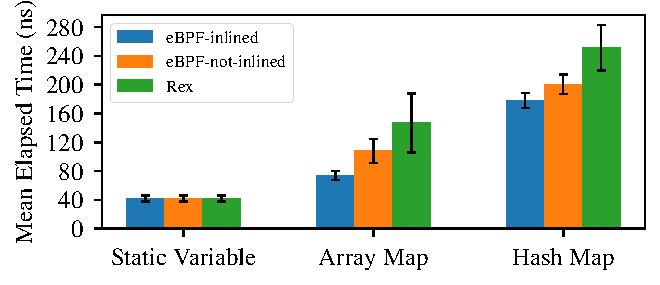
\includegraphics[width=1.0\linewidth]{figs/inline.pdf}
    \centering
    \vspace{-25pt}
    \caption{Runtime of map lookups on various setups}
    \label{fig:eval-inline}
    \vspace{-10pt}
\end{figure}

% \begin{itemize}
%     \item inline v.s. out-of-line map helpers
%         \begin{itemize}
%             \item table showing runtime of a map lookup operation in a eBPF and
%                 a Rust program
%             \item the kernel will automatically inline lookup in BPF
%             \item Rust version will not get inlined
%             \item measurement can be in ns for now, but better if it could be
%                 in cycles
%             \item maps to test: array, hash (htab-lru, xsk-map?)
%         \end{itemize}
% \end{itemize}

We evaluate the impact of missed opportunities due to the elimination of the
    eBPF verifier in \projname{}.
Specifically, we look into the optimization of eBPF map lookups.
For eBPF programs, the verifier can inline the \texttt{bpf\_map\_lookup\_elem}
    helper function by replacing the call into equivalent eBPF instructions.
This optimization can avoid two function calls and two pointer dereferences for
    map types that support lookup inlining.
However, in \projname{}, inlining is not performed due to the absence of the
    eBPF verifier as well as kernel internal information (e.g. map addresses).

In this experiment we measure the runtime of eBPF map lookups under three
    settings, eBPF with inlining, eBPF without inlining, and \projname{}.
Our test program for both eBPF and \projname{} is a tracepoint program that
    uses the \texttt{bpf\_ktime\_get\_ns} helper to measure the runtime of
    a \texttt{bpf\_map\_lookup\_elem} call.
The \texttt{bpf\_map\_lookup\_elem} invocation is by defualt inlined by the
    eBPF verifier when possible.
The setup of eBPF without inlining is achieved by removing the inlining logic
    from the eBPF verifier.
We selected two commonly-used eBPF map types for this experiment: array maps
    and hash maps.
Both of them support lookup inlining.

% Figure~\ref{fig:eval-inline}
% shows the performance of inlining and non-inlining on a vanilla
% v5.15 kernel as well as the \projname{} implementation.
Figure~\ref{fig:eval-inline} shows the performance of map lookups under the
    three different setups on different maps.
% The vanilla non-inlined
% kernel is achieved by commenting out the lines in the kernel verifier.c file that
% automatically inlines the bpf\_map\_lookup\_elem method.
For both array maps and hash maps, the
    runtime of map lookup can be reduced by 20-30 ns compared to eBPF without
    inlining.
% In the graph,
% the performance impact of inlining the method is 20-30 nanoseconds.
% The additional slowdown of 30-40 nanoseconds seen in the rust implementation
% can be explained by the wrapping performed around the bpf\_map\_lookup\_elem method.
An additional slowdown of 30-40 nanoseconds is present for map lookups in
    \projname{}.
This is because of the wrapping code around the kernel
    \texttt{bpf\_map\_lookup\_elem} that allows \projname{} programs to invoke
    it using safe Rust objects.

% Egor: Not sure if I should go into more technical details about whats going on
% in the wrapping

% Using libbpf (and libiu in the case of \projname{}) the sample \projname{} or c bpf
% program is loaded and attached to a tracepoint which is then called by the trigger.
% In the instance of the inlined and non-inlined tests this tracepoint is getcwd, and
% in the instance of the rust tests that tracepoint used is sys\_enter\_dup. The
% triggers consist of a one-line c program that calls the appropriate function such as getcwd().
% The bpf program creates the corresponding map and measures the time
% it takes to execute a single map\_lookup\_elem. This time is measured with
% bpf\_ktime\_get\_ns() and then printed with bpf\_printk() and recorded.
% \milo{Maybe we should talk about why we chose these specific maps. i.e. that array and hash maps are the main ones that support the inlining?}

\subsubsection{Stack-check overhead}
\begin{itemize}
    \item table showing runtime of two programs using small recursion
    \item eBPF: use tail calls for recursion
    \item Rust: just a recursive function
    \item The recursion count should not be statically known to prevent llvm
        from optimizing out the recursion
\end{itemize}

We then evaluate how much overhead the runtime stack check have on the
    performance of \projname{} programs.
The stack instrumentation is added before each
    function call in the \projname{} program if the program contains indirect
    or recursive function calls that prevents the compiler from calculating the
    stack usage statically.
In this experiment we implement recursive factorial computation program in both
    eBPF and \projname{}.
Since eBPF does not natively support recursive functions, we use eBPF tail
    calls to invoke the same program.
At same time, because recursive factorial computation can always be tail-call
    optimized in Rust, this comparison should be able to precisely highlight
    the performance implication of the runtime stack instrumentation.
\jinghao{TODO: discuss results.}

\subsubsection{Cleanup overhead on normal execution path}
\begin{table}[t]
    \small
    \centering
    \begin{tabular}{cc}%{|p{6cm}|p{1cm}|}
        \toprule
        \textbf{Extension} & \textbf{Runtime of acquiring \& release a lock (ns)} \\
        \midrule
        eBPF & 256.8 $\pm$ 142.4 \\
        \projname{} & 254.5 $\pm$ 192.3 \\
        \bottomrule
    \end{tabular}
    \caption{Runtime of spinlock acquire and release for eBPF and \projname{}}
    \vspace{-10pt}
    \label{tab:cleanup-overhead}
\end{table}

The cleanup mechanism employed by \projname{} requires recording the allocated
    resource at runtime, which comparing to eBPF or Itanium C++ ABI, adds extra
    runtime overhead.
We therefore evaluate the runtime overhead from \projname{}'s cleanup
    mechanism.
For this miscrobenchmark, we choose to use a program that acquires and then
    immediately releases a BPF spinlock.
Since the acquired spinlock is a resource that needs to be released upon Rust
    panics, \projname{}'s cleanup mechanism needs to record it in its per-CPU
    buffer.
The program is implemented both in eBPF and \projname{} and the time used to
    acquire and release the spinlocks are measured.
As shown in Table~\ref{tab:cleanup-overhead}, the runtime difference between
    eBPF and \projname{} is less than 2ns with \projname{} being the faster
    one, implying the overhead of \projname{}'s cleanup mechanism is
    negligible.

\subsection{Macro-benchmarks}
\label{eval:macro}
We now demonstrate that \projname{} can be used to implement complicated,
    real-world kernel extension use cases with enhanced usability but without
%    losing much performance by implementing BMC and Electrode in \projname{}.
    losing much performance by implementing the BPF Memcached Cache (BMC) in
    \projname{}.

% \subsubsection{\projname{}-based BMC}
% \jinghao{TODO: Preamable}
% BMC implements in-kernel memcached cache -- how it works
% Compilcated program, original paper splits into 7 programs and uses tail calls
%

BMC~\cite{BMC} is an in-kernel cache for Memcached based on eBPF.
It stores recently queried key-value pairs in an eBPF map to accelerate the
    processing of GET requests to the Memcached server.
If a GET is hit in the cache, the queried value can be sent in a reply without
    going through the expensive network stack in the Linux kernel.
The map that servers as the cache is managed by eBPF programs, which implements
    the lookup and update logics.

On the aspect of implementation, BMC is a much more complicated program
    comparing to other common eBPF use cases.
In order to pass the verifier, the implementation has to be splitted into seven
    eBPF programs that tail-calls into each other to reduce verification
    complexity.
Similar problem also presents when processing the incoming packet data, where
    the authors had to bound data size to reduce verification complexity for
    loops.

We re-implement BMC in \projname{} (\projname{}-BMC) to demonstrate the
    enhanced usability without losing performance.
The resulting program is not a direct translation from the original eBPF
    version in C, rather, we implement the same high-level logic but with
    slight deviations from BMC where the enhanced usability and expressiveness
    of Rust allows a simpler implementation.

% The BMC has many places where for loops are nested into different ifs.
% And, due to the limitations of C, many operations do not have built-in functions
%     that can be used directly.


In the initial design of \projname{}-BMC, the underlying assumption was that
    we should follow the logic of BMC.
But the cache invalidation function in BMC employs
    for loops with cumbersome condition checks, and is further
    complicated by the nesting of multiple if statements.
The complexity is exacerbated by introducing two additional variables to track
    special states.
\jinghao{What states? It does not need to be too detailed.}
Such complex conditional judgments will significantly undermine the readability
    of the BMC code, and it may lead to ambiguities in some places regarding
    the intended functionality.
\jinghao{Can we make the claim that this complexity is for passing the
    verifier?}
% During implementation of function \texttt{bmc\_invalidate\_cache},
%     we assume that each pcket

% However, subsequent testing revealed the possibility of multiple set commands
%     within a single packet.

% This discovery highlighted the obscurity and susceptibility to errors inherent
%     in the original code structure, primarily due to the complex judgment
%     conditions buried within nested if statements.

To address these challenges, \projname{}-BMC utilizes the lazy-evaluated
    \texttt{filter\_map} function from Rust iterators.
\jinghao{What are these challenges -- are we still in the context of cache
    invalidation? By the way, can we abstract this out to all ``loops'' in BMC?
At the same time, we probably need to explain what \texttt{filter\_map} does.}
This approach facilitates the creation of an iterator, which is instrumental in identifying
    the quantity of SET commands present in the current packet payload.
Further enhancing the readability, Rust's syntactic sugar is employed for
    iterating over the identified memcached SET commands, streamlining the process.
The complexity of the original code, characterized by four levels of nesting,
    is significantly reduced by converting a for-loop with intricate conditions
    into a lambda function.
\jinghao{lambda function -> a clean chain of higher-order functions with
    lambda function?}
This conversion is achieved through the utilization of \texttt{take\_while}
    combined with generated iterator, thus dividing the code into three distinct
    sequential parts and markedly improving its expressiveness.
\jinghao{Also should explain what \texttt{take\_while} does.}

\jinghao{Now it feels like we should make part larger, i.e., include code
    examples and show how Rust helps with that.
We can then move this part into the new qualitative evaluation.}

%\para{Experiment setup}
Our evaluation setup consists two machines, with one
    acting as the server and the other one acting as the client.
The server machine runs the \projname{} custom kernel based on Linux v5.15.0 on
    an AMD EPYC 7551P 32-Core processor with 112 GB memory.
SMT and Turbo are turned off for the experiments.
The client machine runs a vanilla v6.8.0 Linux kernel on AMD Ryzen 9 7900X
    processor with 128 GB memory.
Both machines are equiped with Mellanox ConnectX-3 Pro 40GbE NICs and are
    connected back-to-back using a single port.

% Key: 16 bytes, value: 32 bytes
% 50 million with Zipf 0.99
% 10 GB memcached, 2.5 GB BMC
% Preload all keys
% GET:SET 30:1

We use the following workload to evaluate our \projname{}-BMC together with the
    original eBPF-BMC.
Our dictionary contains 50 million Memcached keys following a Zipf
    distribution with 0.99 skewness.
All keys are 16 bytes in size and are paired with 32-byte values in the
    experiments.
The storage sizes of the Memcached and BMC are set to 10 GB and 2.5 GB,
    respectively.
According to the calculation in the original work, all items
    can be stored in Memcached itself but only 6.3 million of them can fit in
    BMC.
Before experiments, the Memcached server is pre-loaded with all keys by
    sending TCP SET requests for each key in the dictionary from the client.
The client then sends requests to the server with a 30:1 ratio betweren UDP GET and
    TCP SET requests and measures the throughput.

We evaluate the throughput of three setups: MemcachedSR (from BMC),
    MemcachedSR+BMC, and MemcachedSR+\projname{}-BMC.
The original open-sourced BMC code targets Linux kernel version 5.3.0 and we
    port it to the v5.15.0 \projname{} kernel for the evaluation.
For each setup, we vary the number of processor cores and the number of threads
    used by the Memcached server and pin each thread onto each core.
We also adjust the CPU affinity of IRQs associated with the NIC such that the
    network interrupts are processed on the same set of cores the Memcached
    server executes on.

\begin{figure}
    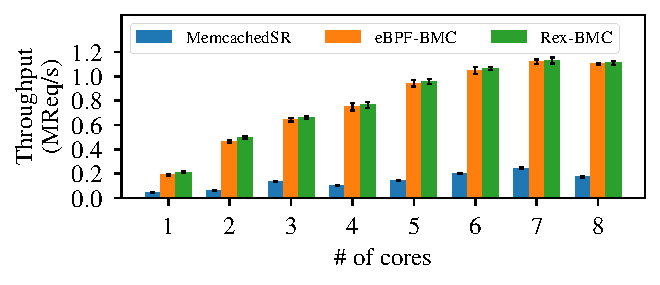
\includegraphics[width=1.0\linewidth]{figs/bmc.pdf}
    \centering
    \vspace{-25pt}
    \caption{Throughput of BMC on MemcachedSR, eBPF-BMC, and \projname{}-BMC
        under different number of CPUs/threads.
    }
    \label{fig:eval-bmc}
    \vspace{-10pt}
\end{figure}

Figure~\ref{fig:eval-bmc} shows the throughput of the three setups under
    different numbers of CPUs and threads.
MemcachedSR processes all requires in userspace and thus its throughput suffers
    from the overhead of the kernel network stack, achieving only 45K requests
    per second under a single thread and 175K requests per second under 8
    cores.
On the other hand, both eBPF-based and \projname{}-based BMC are able to
    achieve a much higher throughput because they can process a large
    fraction of requests at NIC level and without the need of going through
    the expensive kernel network stack.
With 8 CPU cores and threads, eBPF-BMC and \projname{}-BMC achieve a thoughput
    of 1.106M and 1.111M, and a performance benefit of 6.3x and 6.4x,
    respectively.
It is also clear that \projname{} is able achieve a better usability while
    keeping the same level of performance and safety guarrantee comparing to
    eBPF,  as the throughput of \projname{}-BMC is comparable to that of
    eBPF-BMC under all CPU/thread setups.

\section{Discussion}
\begin{itemize}
    \item Unsafe code in rt crate
    \item Verified Rust extension using Verus
    \item Dynamic allocation (if we end up not doing it)
    \item Cross-Language Attacks from NDSS 2022
    \item Rust memory ordering in kernel (\url{https://lwn.net/SubscriberLink/967049/66bfb6f365d164aa/})
\end{itemize}
\section{Related Work}
\subsection{Rust-based system}
\begin{itemize}
    \item Theseus
    \item Redleaf
    \item Evolving Operating Systems Towards Secure Kernel-Driver Interfaces
    \item Michael Swift works
    \item Leveraging Rust for Lightweight OS Correctness
    \item Cross-Language Attacks from NDSS 2022
\end{itemize}

%\subsection{Other eBPF safety}
\subsection{Unprivileged eBPF through Extra Safety}
Other work has attempted to add additional safety to eBPF programs largely
    to support unprivileged eBPF.
MOAT~\cite{lu2023moat} uses hardware based Intel Memory Protection Keys
    to isolate eBPF programs from the kernel.
This would prevent attackers from using eBPF.
Another system SandBPF~\cite{sandbpf} uses software fault isolation to dynamically
    sandbox eBPF programs.

\subsection{Other OS extension}
A large body of work exists around the theme of creating extensible operating systems.
Systems such as SPIN \cite{spin} utilize the type safety of Modula-3 to produce safe extensions that dynamically link into the kernel.
VINO \cite{vino} uses software fault isolation techniques and interposition to allow for kernel functions to be replaced, or event-based extensions to be implemented.
Similarly, SLIC \cite{slic} uses interposition as a mechanism to allow trusted extensions to be run with only minimal operating system changes.

\section{Conclusion}
This paper identifies the fundamental \gap{} within the current Linux eBPF
    infrastructure that is the source of its poor usability.
We make the observation that by using a safe language for kernel extensions and
    remove the extra verification layer, both the desired usability and safety can be
    achieved.
We demonstrate this by presenting \projname{}, a Rust-based kernel extension
    framework for the Linux kernel that leverages language-based safety from
    Rust without a separate verfier.
We show that \projname{} is able to solve existing usability issues
    associated with the eBPF verifier without performance costs, facilitating
    safe and easy-to-write kernel extensions.
%%
%% The next two lines define the bibliography style to be used, and
%% the bibliography file.
\bibliographystyle{acm}
\bibliography{ref}

% \appendix
% \appendix
\section{Appendix}
% \label{sec:impl}

\jinghao{\S\ref{sec:impl}: How to make it work}

% \subsection{Design goal}

%\begin{itemize}
%     \item Safety
%         \begin{itemize}
%             \item Same level of safety as eBPF
%             \item Memory safety
%             \item Control-flow soundness
%             \item Resource management
%             \item Program termination
%         \end{itemize}
%     \item Expressiveness
%         \begin{itemize}
%             \item Support more complicated/advanced programs
%             \item Longer programs
%             \item Unbounded loops
%         \end{itemize}
%     \item An important note: we want expressiveness w/o impairing safety (e.g.
%         allow unbounded loop while ensuring termination)
% \end{itemize}

% \subsection{Overview}
% \begin{itemize}
%     \item Brings out the Rust based approach (use Jiyuan's property-oriented
%         argument: We want these properties, and Rust happens to provide these)
%     \item Infrastructure (Need a figure similar to Fig. 5 from HotOS paper)
% \end{itemize}

We now discuss the high-level mechanisms that we use to build various features in
    \projname{} and make it a practical kernel extension framework.
These include the following:
\begin{itemize}
    \item How the \projname{} kernel crate bridges programs and the kernel.
    \item How \projname{} programs are loaded and attached.
    \item How eBPF maps are supported in \projname{}.
    \item How is the entry of \projname{} implemented that allows kernel to
        execute them directly.
\end{itemize}

\subsection{\projname{} kernel crate}
% \begin{itemize}
%     \item overall structure: program type, kernel binding generation, wrapper
%         interface around binding.
%     \item context conversion
%     \item kernel helper and symbol bindings (dynamic linking scheme)
%     \item kconfig-based conditional compilation
%     \item Map support
% \end{itemize}

The \projname{} kernel crate is responsible for supporting interactions between
    kernel and \projname{} programs and contains interfaces facing both sides.
% It contains support for different program types with
%     interfaces facing the kernel and the \projname{} program.
\projname{} support the same set of program types as eBPF.
Each program type is defined as a Rust struct and with allowed helpers defined
    as its methods.
This effectively implements access control on helper functions with respect to
    program types (e.g., a tracing program should not modify socket buffers
    through networking helper functions), which is also present in eBPF.
The user defines a program object of one of the program struct types and
    assoociates it with a Rust function as the extension program.
The extension function takes in the associated program object and the
    program-type-specific context from the kernel as arguments
    (\S\ref{impl:ctx-converison}).
Inside the extension, developers can use Rust kernel bindings generated by the
    crate to access kernel structures (\S\ref{impl:crate:binding}).
At the same time, helper functions allowed for the program type can be
    invoked through the program object, which are backed by eBPF kernel helpers.
    (\S\ref{impl:crate:symbol-resolv}).

% The crate also has support for maps (\S\ref{impl:map}) and other
%     miscellaneous utilities for the ease of programming (e.g. wrapping return
%     code in \texttt{Result} to support monadic operations in Rust).

\subsubsection{Supplying program context}
\label{impl:ctx-converison}
% Like eBPF, \projname{}
Extension programs take in a kernel-provided ``context'' as input argument.
The context is a pointer to a struct that contains information the program may
    need.
The current eBPF keeps a pair of context struct definitions for certain program
    types, where one of them is exposed to extension programs and the other one
    is the internal data structure in the kernel.
The extension-facing definition is generally a subset of the associated kernel
    internal definition.
This is done for the reason of keeping a stable interface and hidding unneeded
    kernel data from the extension programs.
When a eBPF program is loaded into the kernel, the verifier rewrites accesses
    into the corresponding field in the kernel context
    through the verifier hook specific to the program type.
Rewriting the access also avoids the need for copying data and contructing an
    extension-facing context.

% In \projname{}, the Rust compiler takes the place of the eBPF verifier and as
%     a result there is no way to rewrite the access to the context the same
%     way eBPF does.
In \projname{} the removal of the verifier means it cannot rewrite the access
    to the context the same way eBPF does.
Instead, \projname{} take the advantage of the expressive Rust language
    features.
In particular, \projname{} exports to the extension programs a struct that just
    wraps around the pointer to kernel context.
It implements accesses to the needed fields in the kernel context as safe Rust
    methods of this struct, which accesses the kernel struct internally via
    generated bindings (\S\ref{impl:crate:binding}).
% Doing so effectively re-route accesses to the kernel struct.
At the same time, it also allows controlled access to the kernel context and
    prevents unwanted writes to the context, which may corrupt kernel data
    accidentally.

\subsubsection{Creating Rust bindings of kernel structs}
\label{impl:crate:binding}
Extension programs rely heavily on the kernel data structure definitions.
A tracing program may want to obtain information from the kernel
    \texttt{task\_struct}, while a networking program needs to know the layout
    of protocol headers.
In eBPF, the need can be easily full-filled by including the corresponding
    kernel header files, as most of the time the program is implemented in C
    and compiled to eBPF bytecode.

The problem becomes more involved in \projname{}, as it uses Rust as the
    programming language, which cannot directly work with kernel C headers.
% As a solution, \projname{} creates Rust bindings for the needed kernel
%     definitions.
As a solution, \projname{} uses Rust-bindgen~\cite{bindgen} to create Rust
    bindings for kernel structure definitions and constants from kernel header
    files.
\projname{} integrates the binding generation into program compilation so that
    the bindings are automatically generated for the target kernel during
    build.
The generated Rust binding forms part of the kernel crate and can be imported
    into \projname{} programs like other contents of the kernel crate.

\subsubsection{Supporting kernel helper functions}
\label{impl:crate:symbol-resolv}
Kernel extensions utilizes kernel helper functions for perform more advanced
    operations.
eBPF uses kernel helpers as both a way to interact with the kernel and to
    complement its limitation on expressiveness.
\projname{}, on the other hand, only uses helpers for kernel interaction, since
    Rust is expressive enough that it does not need additional helper functions.

\projname{} uses the existing eBPF helper interface and implements on top of
    it a Rust wrapping layer.
This wrapping layer serves to hide the unsafe kernel C helper interface and
    provides a new interface that \projname{} programs can safely use.
The implementation of eBPF map lookup helper is shown in
    Figure~\ref{fig:map-helper}.
On L30, the kernel helper function returns a pointer to the map value
    (\texttt{*mut V}), the \projname{} wrapping layer converts the pointer
    into a Rust option type~\cite{rust-option} (\texttt{Option<\&mut V>}) on
    L33-L37, which allows \projname{} programs to access the object through a
    safe Rust reference without worrying about deferencing a null pointer.

\begin{figure}[t]
    \lstinputlisting[language=Rust]{./snippets/s5-map.rs}
    \vspace{-10pt}
    \caption{Implementation of eBPF map support in \projname{}}
    \vspace{-10pt}
    \label{fig:map-helper}
\end{figure}

In eBPF, most of the helper calls are direct function calls, however, a few of
    them are further optimized during verification and JITing.
Helper functions in \projname{} do not have the same load time optimization,
    and at the same time the kernel crate wraps the unsafe kernel helpers with
    a safe Rust interface, which could incur further overhead.
We further evaluate the impact in \S\ref{eval:inline}.

% For required kernel symbols (e.g., kernel helper functions), the kernel crate
%     creates a stub declaration for each symbol without using Rust-bindgen.
% This is because certain kernel symbols -- especially all eBPF helper
%     functions --  do not have a declaration in kernel header files.
% The actual definition of the kernel symbols will be resolved when the program
%     is loaded into the kernel (\S\ref{impl:crate:symbol-resolv}).

% The \projname{} kernel crate serves as an interface for the extension programs
%     to interact with the kernel.
% To accomplish this, the crate will need to access kernel symbols.
To reuse the existing kernel helper interface, the crate will need to access
    kernel symbols.
At the same time, the crate itself may also need to access certain kernel
    symbols for internal house keeping operations (e.g. resource cleanups as in
    \S\ref{principle:eh})
% For example, invoking kernel helper functions requires knowing the kernel
%     address of the target helper function symbol.
% These kernel symbols includes not only BPF helper functions, but also other
%     global and per-CPU variables.
Because \projname{} programs are compiled in userspace, the compiler does not
    have any knowledge on the required kernel symbols.
% One simple solution is to directly passing kernel symbols and their
%     corresponding addresses to userspace (e.g. through \texttt{/proc/kallsyms})
% However, this is in general considered a dangerous practice as it leaks kernel
%     addresses to userspace.
% At the same time, this solution is not robust against kernel layout changes
%     (e.g. due to kernel rebuild) -- changes of a kernel symbol address requires
%     a recompilation of the \projname{} program that uses it.

\projname{} therefore defers the kernel symbol resolution to program load time,
%     i.e., when the compiled \projname{} program is sent to the kernel.
    the same way dynamic linking works in userspace.
At this point, the booted kernel always knows where the symbols are located.
%     even after layout changes.
% At the same time, the sensitive kernel addresses do not need to be leaked to
%     userspace.
% \projname{} implements this kernel symbol resolution scheme the same way
%     dynamic linking works in userspace.
The \projname{} kernel crate merely creates stub declarations for the required
    kernel symbols.
During compilation, the compiler treats all kernel symbols as external and
    generate relocation entries for the undefined symbols.
At load time, the loader library (\S\ref{impl:load}) parses the executable,
    compiles a list of kernel sybmols that require resolution with their
    corresponding entries in the global offset table (GOT), and sends the
    information to the kernel.
The kernel then resolves the address for each symbol via the kallsyms subsystem
    and patches the GOT entries with the resolved addresses.
This allows programs to access kernel symbols without the need to disable
    kernel address space layout randomization (KASLR).
% and allows programs to correctly referencing these kernel symbols.

\subsubsection{Kconfig-aware conditional compilation}
% kernel uses config-based conditional compilation
% certain functionalities may not be compiled in
% we also use conditional compilation in kernel crate
% read config from build script and pass to the compilation process
The fact that the Linux kernel employs conditional compilation extensively
    based on kernel configuration values implies that certain functionalities
    used by \projname{} programs may not be compiled in.
An example of this is the ability to override the return value of a function in
    Kprobe programs.
This is only available if the \texttt{CONFIG\_BPF\_KPROBE\_OVERRIDE} is
    enabled, which is checked by the verfier in current eBPF.
The \projname{} kernel crate utilizes the conditional compilation counterpart
    in Rust.
The build script~\cite{rust-build-script} of the crate parses the configuration
    of the target kernel and send configuration values of interest to the
    compiler.
The compiler the conditionally compiles the code guarded by the configurations.
If a functionality does not have its associated configuration set, its support
    in the kernel crate will not be present, either.

\subsection{Program load and attachment}
\label{impl:load}
% \begin{itemize}
%     \item kernel loading code and attachment (w/ base program)
%     \item relocation fixups for maps and kernel symbols
%     \item libiu
% \end{itemize}
% Difference between eBPF and Rust programs
% - native code vs. byte code + JIT
% - no verifier to fixup relocations for maps and kernel symbols (e.g helpers)
% Implement kernel side loading logic
% - allocate page and map all LOAD segments in the ELF executable
% - fix all relocations for maps and kernel symbols
% - use the same eBPF insfrastructure
% problem where programs within the same executable share code
% - multiple programs calling the same function
% - one copy per program is ineffcient on memory
% - solution: first load the ELF executable, then associate individual programs
%   with extension entry functions in the code
There are two major differences between eBPF and \projname{} that poses unique
    challenges to the loading of \projname{} programs in the kernel.
Firstly, \projname{} is loaded as native code after compilation, of which the
    kernel does not have control on the layout.
This means the kernel need to parse and handle different sections in the
    program differently.
In contrast, eBPF is loaded as eBPF bytecode and contains only executable code.
The kernel has complete control over the generated native through the kernel
    eBPF JIT infrastructure.
Secondly, \projname{} does not have the in-kernel verifier, which is used in
    eBPF to fixup the kernel objects the program references (e.g., maps and
    helpers).
Therefore, the loading logic also needs to perform fixups needed for
    \projname{} on relocations.

The loading of a \projname{} program can be divided into two phases, with the
    first one happening in userspace and the other in kernel space.
The first phase is responsible for parsing the ELF executable into a format the
    kernel can understand as well as performing prerequisite operations (e.g.,
    creation of eBPF maps).
In \projname{} this is done by its userspace loader library \texttt{librex}.
Similar to how \texttt{libbpf} operates on eBPF programs, \texttt{librex}
    provides routines that parses the eBPF maps, kernel symbol relocations,
    and programs from the \projname{} ELF executable.
Once the sections are parsed, it creates the eBPF maps and update the
    corresponding map entries in the ELF (\S\ref{impl:map}), and then load
    the program by sending the ELF binary as well as the map and relocation
    information.
Parsing the ELF sections in usrspace avoids complexity of the loading logic in
    the kernel.

For the second phase, we extend the \texttt{bpf} system call to support loading
    of \projname{} programs.
The system call sends the compiled ELF executable as well as the associated
    relocation information into the kernel.
The kernel first parses the ELF executable and locate all the \texttt{LOAD}
    segments in the executable.
It then allocate new pages and maps the \texttt{LOAD} segments into the
    kernel address space based on the size and permissions of the segments.
With the associated relocation information, the kernel updates the kernel
    symbol relocation entries (\S\ref{impl:crate:symbol-resolv}) and eBPF maps
    (\S\ref{impl:map}) with the corresponding absolute address in the kernel.
% The relocations that need fixup are kernel symbols referenced by the
%     \projname{} program (\S\ref{impl:crate:symbol-resolv}) and eBPF maps
%     (\S\ref{impl:map}).
At this point, the program is considered ``loaded''.
The kernel then wrap the program into a \texttt{bpf\_prog} struct as if it is a
    JIT-ed program -- reusing the existing eBPF infrastructure for program
    management greatly reduces engineering efforts and facilitates easy
    integration with existing eBPF hook points.

Kernel extensions often involves use cases where multiple programs are defined
    together and share common code in the same executable.
% One of the problem \projname{} faces is to deal with multiple programs within
%     the same ELF executable.
% Such programs may share common code in the same executable.
eBPF loads each of the program independently and deplicates the shared code. \jinghao{need check}
% It is obviously not memory efficient if the load of each program requires
%     loading and mapping of the same executable.
This is obviously not memory efficient for \projname{} because duplicating
    shared code means duplicating the \projname{} kernel crate.
The soluation \projname{} uses is that it separates the steps of mapping the
    executable into kernel memory and loading of programs.
The userspace first invokes our extended \texttt{bpf} system call to map the
    whole executable into kernel address space and obtain a reference count to
    the mapped code (behind a file descriptor).
It then can invoke the syscall again to load the program into the kernel.
This later step is simple as it only needs to wrap the function associated with
    the \projname{} program into the \texttt{bpf\_prog} struct.
The newly created \texttt{bpf\_prog} struct takes the reference count of the
    mapped executable code so that the kernel will not clean it up before the
    programs are destroyed.
This allows multiple programs to effectively share the same executable code and
    avoid waste of memeory resources.

\subsection{Supporting eBPF maps}
\label{impl:map}
% maps are important: storage and data sharing
% supporting map is hard:
%   2 step of rewriting for the sake of easy programming and hide kernel
%     pointer
%   Not directly available in Rust
%   need to make map interface safe
%   also need seamless support as eBPF does
%
% Use a loader library:
%   define a ABI of Rust map object in memory (metadata + actual kptr) put in
%     .map section
%   loader library parse elf object and find all maps
%   use the defined ABI to read out metadata and create map via bpf syscall
%   rewrite kptr in each map in the elf object with map fd (safe because
%     kptr is 8 byte and can be treated as an int and map fd is 4 byte)
%   when loading the program, send in the updated elf object and offset of each
%     map kptr within the object
%   kernel will use the previously written fd in the kptr to retrieve the real
%     address of the map and update kptr value.
%   kptr is initialized to null, since compiler does not see the post
%     compilation fixups, it will assume the value never changes and
%     constant-propogate the map kptr, leading to incorrect program behavior
%   e.g. the map helpers always verifies the kptr is not null before invoking
%     actual kernel helper, assuming the kptr to be always null makes the map
%     helper always return error without calling into the kernel
%   solution: treat the kptr as a volatile variable and force a load before
%     each map call
%
The kernel eBPF maps provide a powerful primitive for extension programs to
    store data across program execution and to easily share data with userspace.
Therefore, such a functionality is highly desired in \projname{}.

Current eBPF allows user to define a eBPF map in the program by defining a
    struct instance that contains the map metadata (e.g. key/value type, number
    of entries) in a specific ELF section for maps.
All map operations on this map would be made through this instance.
At program load time, \texttt{libbpf}, the eBPF loader library, parses the map
    metadata from the struct instance.
It then creates the map in the kernel through the \texttt{bpf} system call and
    obtain a file descriptor referring to the map.
\texttt{libbpf} rewrites the eBPF bytecode such that all references to the
    created map are updated to the value of the file descriptor.
When the program is loaded to the kernel, the eBPF verifier performs a second
    round of rewriting -- for each map file descriptor, it obtains the actual
    kernel eBPF map struct the file descriptor refers to and updates the
    references to the address of the kernel internal map struct.
This two-stage rewriting provides two desired properties: it 1) prevents
    leaking of a kernel map address to userspace and 2) allows seamless and
    transparent interaction with the kernel maps from extension programs.
However, supporting eBPF maps in the ways of eBPF is not trivial in
    \projname{}, because the ABI of map metadata struct is eBPF-specific and
    the absence of in-kernel verifier.
% However, for \projname{}, achieving these two properties is not trivial: the
%     Rust compiler cannot provide these since creating maps is out-of-scope for
%     compilation, and at the same time the existing two-stage rewriting is specifically
%     for eBPF and cannot be reused for Rust programs directly.

In order to support a safe and convenient map interface, \projname{} defines
    its own ABI for storing map metadata and implements the rewriting logic in
    its own program loader library and kernel program loading code.
In \projname{} programs, users can define a map by creating a new, static
    \texttt{RexMap} object in the \texttt{.map} section through a convenience
    macro provided by the \projname{} kernel crate.
Part of the implementation of \texttt{RexMap} is shown in
    Figure~\ref{fig:map-helper}.
\texttt{RexMap} is exported by the \projname{} kernel crate, which contains
    various map parameters, and a private pointer to the kernel map struct.
The struct uses generic types to encode the map type, key type, and
    value types.
All map helpers in \projname{} are also generic functions with the same set of
    generic parameters, which take \texttt{RexMap} objects as arguments and
    internally invoke the kernel map helper functions with the kernel map
    pointer.
Doing so ensures safety of map operations -- it prevents mismatches in map
    types and key/value types (\S\ref{principle:memsafety}).
The creation of \texttt{RexMap} is set to be constantly evaluated; in other
    words, this means its fields are initialized at compile time and readily
    available in the executable data.
This is the same as how eBPF initilizes ``legacy'' maps (newer maps are
    initialized via BTF debug information).

The ABI is implemented by forcing the \texttt{RexMap} struct to have
    C-representation~\cite{nomicon-reprc}, i.e., the memory layout
    is the same as a equivalent C structand thereby enforce a stable layout.
Doing so allows \texttt{librex}, the \projname{} loader library to easily parse
    a \texttt{RexMap} struct to obtain the map metadata.
Similar to \texttt{libbpf}, \texttt{librex} finds and parses all maps in the
    \texttt{.map} section.
% This is possible because the constructor of \texttt{RexMap} is defined as
%     a constant expression and therefore the \texttt{RexMap} objects are
%     initialized at compile time.
With the metadata for each map, the library creates the requested eBPF maps in
    the kernel using the \texttt{bpf} system call and rewrites the kernel
    pointer field of each \texttt{RexMap} object to the file descriptor value.
When loading the program, the loader library sends both the updated ELF
    executable and a list of offsets of the kernel map pointer field within the
    executable to the kernel.
The kernel reads the file descriptor at each offset and update it with the real
    map address referred by the file descriptor to make all map operations
    work.

During compile-time initialization, the kernel pointer field in
    \texttt{RexMap} is set to a null pointer.
Since the \texttt{RexMap} objects are defined as read-only and rewriting
    happens after compilation, this makes the Rust compiler incorrectly assume
    the kernel map pointer always stays \texttt{NULL}.
This in turn causes the compiler to perform constant propagation on the kernel
    pointer field when optimizations are enabled, leading to incorrect program
    behavior.
For example, the \projname{} map helpers in the \projname{} kernel crate always
    verifies that the kernel pointer is not null before invoking the kernel map
    helper functions.
By constant-propagating the \texttt{NULL} pointer value, the compiler believes
    the check always fails and makes the map helper always to return error
    without calling into the kernel helper function.
In order to solve this problem, the \projname{} kernel crate treats the kernel
    pointer as volatile and forces a load of the pointer value from memory
    every time it is used by the map helpers.
\jinghao{Feels this paragraph does not add much, shall we remove it}

\subsection{Safe guarding program entry}
% \begin{itemize}
%     \item LLVM pass
% \end{itemize}
To allow \projname{} extension code in Rust to be called from the kernel C
    code, an FFI entry-point function is needed to wrap around the user-defined
    extension function.
This wrapper function needs to handle certain unsafe operations, including
    interpreting the context argument supplied by the kernel as a Rust
    reference and performing context conversion for selected program types.
Because of this, this entry function should not be implemented by the user.
For example, interpreting an XDP context as a kernel perf-event context and
    perform the context conversion specific to perf-event would violate memory
    and type safety and result in undefined behavior.
Therefore, \projname{} chooses to automatically generate the entry point code
    during compilation of the Rust extension programs.

We implement the generation of entry code as an compiler pass, taking the
    advantage of Rust's use of LLVM as its code generation backend.
At the LLVM-IR stage, the entry code generation pass reads out the information
    related to the program from the program object the user defines.
This is achieved by implementing a similar ABI to \texttt{RexMap}s
    (\S\ref{impl:map}) on program objects, which creates a fixed memory layout
    of the program object
% This is achieved by enforcing a specific memory layout of the program object
%     struct (e.g., always store the program type in the first integer field) and
%     then constant-initializing the program object, which effectively implements
%     an ABI between the Rust compiler front end and the LLVM middle/back end.
The pass generates a new entry function for the program.
%     with the
%     user-supplied program name.
The function has the same prototype as the in-kernel hook point, and therefore,
    the kernel can directly invoke the function from the place the program is
    attached.
Inside the entry function, depending on the type of the program, the pass
    generates code that invokes the program-type-specific code from the
    \projname{} kernel crate that dispatches the program.
The code reinterprets the context argument supplied by the kernel into a Rust
    object, performs context conversion if needed
    (\S\ref{impl:ctx-converison}), and eventually call into the
    user-defined extension function that is associated with the \projname{}
    program object.

% \subsection{Handle exceptional control flow}
% \begin{itemize}
%     \item kernel trampoline
% \end{itemize}

% \subsection{Stack overflow protection}
% \begin{itemize}
%     \item kernel vmapped, dedicated stack
%     \item LLVM instrumentation
% \end{itemize}


\end{document}
\endinput

